\documentclass{llncs}
\usepackage{graphics}
\usepackage[dvips]{epsfig}
\usepackage[latin1]{inputenc}
\usepackage{color}
\usepackage{longtable}
\usepackage{multirow}
\usepackage[dvips]{graphicx} 
%\usepackage{pgfplots}
%\usepackage{amsmath}
\usepackage{textcomp}
\usepackage{url}

\newcommand{\tab}{\hspace{20mm}}

\setlength{\textfloatsep}{8pt plus 2pt minus 2pt}
\setlength{\intextsep}{8pt plus 2pt minus 2pt}

%#\def\BibTeX{{\rm B\kern-.05em{\sc i\kern-.025em b}\kern-.08em
%#    T\kern-.1667em\lower.7ex\hbox{E}\kern-.125emX}}

%\hyphenation{}


\begin{document}

%%%%%%%%%%%%%%%%%%%%%%%%%%%%%%%   TITLE   %%%%%%%%%%%%%%%%%%%%%%%%%%%%%%%

\title{Designing and Evolving an Unreal Tournament\texttrademark~2004 Expert Bot}
%\thanks{\footnotesize{This paper has been funded in part by project TIN2011-28627-C04-02 and project P08-TIC-03903 awarded by the Andalusian Regional Government.}}}

\titlerunning{Evolving an UT2K4 Expert Bot}

%%%%%%%%%%%%%%%%%%%%%%%%%%%%%%%   AUTHORS   %%%%%%%%%%%%%%%%%%%%%%%%%%%%%%%

\author{A.M. Mora \and F. Aisa \and R. Caballero \and \\ P. Garc�a-S�nchez \and J.J. Merelo \and P.A. Castillo}
\authorrunning{A.M. Mora et al.}

\institute{Departamento de Arquitectura y Tecnolog\'{\i}a de Computadores.\\
Universidad de Granada (Spain)\\
\email{\{amorag,jmerelo,pgarcia,pedro\}@geneura.ugr.es, francisco\_aisa@hotmail.com, rcabamo@gmail.com}
}

\maketitle

%
%%%%%%%%%%%%%%%%%%%%%%%%%%%%%%%   ABSTRACT   %%%%%%%%%%%%%%%%%%%%%%%%%%%%%%%
%
\begin{abstract}
This work describes the design of a bot for the first person shooter
Unreal Tournament\texttrademark~2004 (UT2K4), which behaves as a human
expert player in 1 vs. 1 death matches. This has been implemented modelling the actions (and tricks) of this player, using a state-based IA, and supplemented by a database for `learning' the arena. 
The expert bot yields excellent results, beating the game default bots in the hardest difficulty, and even being a very hard opponent for the human players (including our expert).
The AI of this bot is then improved by means of three different approaches of evolutionary algorithms, optimizing a wide set of parameters (weights and
probabilities) which the expert bot considers when playing.  
The result of this process yields an even better rival; however the noisy nature of the fitness function (due to the pseudo-stochasticity of the battles) makes the evolution slower than usual.
% Decid algo del fitness ruidoso y todo eso.
\end{abstract}

%%%%%%%%%%%%%%%%%%%%%%%%%%%%%%%% INTRODUCTION %%%%%%%%%%%%%%%%%%%%%%%%%%%%%%%%%
\vspace{-0.7cm}
\section{Introduction}
\label{sec:intro}
%

A \textit{bot} is an autonomous agent which tries to behave as a human player, normally fighting against some other humans/bots in a computer game. There are different types of bots in addition to the opponents, such as the cooperative players (try to aid the main player). They essentially refer to an
Artificial Intelligence (AI) engine which is able to perform the same actions in a game as a human player.

First Person Shooter games (FPS) are one of the most profitable area in the
study/implementation of bots due to their usual open-code philosophy. They are games where the player can only see the hands and the current weapon of his character, and has to fight against enemies by shooting to them. They usually have a multiplayer fighting mode placed in a limited arena.

Unreal game series follows this philosophy to make it easy the game-modding (modification), including with every copy of the game an editor (UnrealEd), an own programming language (UnrealScript), and a compiler, to add/change almost whatever the user desires: scenarios, items, characters; just with a few constraints. The state-based AI engine is also open.

Moreover, some additional tools have arisen some years ago, such as GameBots\footnote{\url{http://gamebots.sourceforge.net/}}, a \textit{mod} that allows the control of characters (bots) in the game through network connections to other programs. The game sends character's sensory information to the client program, which can decide the actions the bot will take. These actions are sent back to the game which interprets them for the bot movement, shooting, jumping, etc.
It was initially released for the Unreal sequel \textit{Unreal Tournament\texttrademark~(UT)} and later implemented for \textit{UT 2003}.
Over the basis of that tool, it was later launched \textit{Pogamut}\footnote{\url{http://pogamut.cuni.cz/main/tiki-index.php}}, which defines an interface (using GameBots architecture) to program the bots externally using Java. It was implemented for Unreal Tournament\texttrademark~2004 (UT2K4).

These open-code possibilities and external tools are the main reasons why this game environment has been widely considered in the computational intelligence researching field \cite{NN_botshumans_IJCNN2008,Agent_Smith_CEC2009,Mora_Unrealbot_EVO2010}.

This work is also embedded in the UT2K4 environment, and uses Pogamut
for implementing a bot which we have named \textit{UT Expert Bot
  (E-Bot)}. Its behaviour (AI) follows a shape of Finite State Machine (based in two levels of states), that describes a complex set of rules. These rules are based in the knowledge of an UT2K4 Spanish expert player and are focused on \textit{1 vs 1 Death Match battle}. It has been modelled according to his experience, including several tricks, as the humans players do, for getting a better behaviour in the game. 
We have considered the rules defined in the official competitions of UT2K4 for human players, such as: there are some items forbidden (U-Damage), weapons are not respawned and the match runs for 15 minutes, not for a number of frags (number of enemies killed).

Once \textit{E-Bot} has been completely defined and tested (it beats
the default game bots in the hardest difficulty levels), we have
designed some evolutionary approaches based on the application of a
Genetic Algorithm (GA)\cite{GA_Goldberg89} for optimizing the set of
parameters (weights, probabilities, thresholds) which the rules of behaviour
apply, following previous approaches
\cite{Mora_Unrealbot_EVO2010,Mora_UnrealTeams_CIG2010}, but considering an own created behavioural model as the main difference with regard to these works, where the standard AI in the game was improved.

A GA is an algorithm where a population of possible solutions (called individuals) are evolved by means of selection and recombination/mutation to create a new set of candidates that compete using their fitness (quality of adaptation) with the rest of solutions, until a stop criterion (i.e. number of generations) is met. Fitness function is a quality function that gives the grade of adaptation of an individual respect the others. This function usually models the problem to solve.

%The rest of the paper is structured as follows. The state of the art in the related topics is commented is the next section. Then, the expert bot AI is deeply described in Section \ref{sec:unrealexpertbot}, along with the evolutionary based approach in Section \ref{sec:evolution}. The experimental setup, runs and results are presented in Section \ref{sec:experiments}. Finally, in Section \ref{sec:conclusions} the conclusions and future work lines are exposed.


%%%%%%%%%%%%%%%%%%%%%%%%%%%%%%% UNREAL FEATURES %%%%%%%%%%%%%%%%%%%%%%%%%%%%%%%

%\section{Unreal Tournament\texttrademark~2004 Game Features}
%\label{sec:unreal}
%
%As previously commented, Unreal\texttrademark~was a very famous FPS published in 1998 for PCs. It presented a very good single mode, but the multiplayer possibilities gave it (and still give nowadays) a great success. Thus, in 1999 it was released Unreal Tournament\texttrademark, which turned the series to multiplayer-aimed games, having several arenas specifically designed for massive battles between humans and/or bots.
%
%The most successful sequel in this series was Unreal Tournament 2004 (UT2K4), due to the spectacular weapons, the excellent design of scenarios and the amazing opponents' AI, based in states and events, inside a huge Finite State Machine \cite{FSM_Booth} (where plenty of \textit{states} and \textit{substates} are present), and including several \textit{optimized scripts} (predefined actions).
%
%This framework inherited all the features that the first Unreal Engine offered for modders: people who add or change components in the game: such as maps, weapons, items or even bots.
%
%Some of these features are:
%\begin{itemize}
%	\item It includes a proprietary programming language, called \textit{UnrealScript}, which combines the C and Java syntax, with some useful features, such as a garbage collector. It is object-oriented and handles implicit references (every object is represented by a pointer).
%
%	\item This language includes the declaration and handling of         \textit{states}, which are the most powerful feature of the Unreal bots' AI. They model one bot status and behaviour at a time, and are defined as classes. During the game (depending on the bot location and status), the current state of the bot is changed, and the functions defined in/for it are performed. 
%
%	\item In addition to the game, a programming environment, named \textit{UnrealEditor} is included. It makes it easy the management of the hierarchy of classes, as well as the creation of new classes which inherits from the existing ones.
%
%	\item It is possible to change an existing class (mod) by creating another one which inherits from it, and modifying the code for the desired functions or methods.
%
%\end{itemize}
%
%In addition this new engine (Unreal Engine 2.5) fixed some of the drawbacks that UnrealScript had, such as the small number of elements in arrays, the limitations in the number of iterations in loops, or the file input/output.
%
%Moreover there were some projects which created specific tools for interacting with UT and UT2K4 engines, such as the previously commented Gamebots \cite{GameBots} and Pogamut \cite{Pogamut3}. These projects let the user implementing mods (mainly bots), using more powerful and flexible programming languages than the limited UnrealScript, such as Java.
%The latter is the tool we have considered in this work due to its 'simplicity' and proved value in the implementation of bots (it has been widely used by several authors in the literature).
%
%Going back to the game, the most traditional combat mode is \textit{Death Match}, in which the player must eliminate as many enemies as possible before the match ends, avoiding being defeated by other players. 
%Everyone have a limited number of health points, which are decreased as
%he/she gets hurt. If the health counter goes down to 0, the player is defeated, and a \textit{frag} is added to the last player who shot him. After being killed, the player is then respawned (usually in the same place or quite near) in the game.
%A match ends when the termination conditions (typically a limit of frags/kills or time) are reached.
%
%In order to aid players to have success in the match, some elements appear periodically in the arena: \textit{weapons} to defeat the enemies (with limited ammunition, and an associated power), and \textit{items}, that provides the player with some advantages (such as extra health, high jump, invisibility or ammunition, for instance).
%
%This mode is usually played by a number of players/bots up to 32 in the recent games of the saga, but a very interesting one is the \textit{1 vs 1 Death Match} battle. It is considered in the official competitions of UT2K4 for human players and presents some specific rules and constraints, such as: there are some items forbidden (U-Damage), weapons are not respawned and the match runs for 15 minutes, not for a number of frags (number of enemies killed).


%%%%%%%%%%%%%%%%%%%%%%%%%%%%%%  STATE OF THE ART  %%%%%%%%%%%%%%%%%%%%%%%%%%%%%%
%
\vspace{-0.3cm}
\section{State of the Art}
\label{sec:stateofart}
\vspace{-0.1cm}
%

%When they arose (became famous) in the last years of the 80s (with Wolfenstein\texttrademark~in 1987), the FPS games were devoted to single player modes. Later, most of them offered multiplayer possibilities but always against other human players, such as DOOM\texttrademark~in 1988.

Bots have been widely used in games since 1992, when Quake\texttrademark~became the first known game in including autonomous characters. It presented not only the option of playing against machine-controlled bots, but also the possibility to modify them or create new ones. Some AI approaches arose such as the SOAR Quakebot \cite{LairdSOAR}, which modelled a human-like behaviour.

Unreal\texttrademark~appeared some years later, being as stated in the previous section, the first game in including an easily programming environment and a more powerful language, thus plenty of bots were developed. However just a few of them applied metaheuristics or complex AI techniques, and most of these bots were based in predefined hard-coded scripts.

%Nowadays, there are many games that offer similar possibilities, but almost all of them are devoted to the creation of new maps (arenas, battlefields) or characters, being mainly focused on the graphical aspect (such as modifications in their topology or appearance respectively). The sequels of Unreal\texttrademark, named with the surname `Tournament' have followed the open-code philosophy so several researches are based in their environment.

The studies involving computer games and the improvement of some
components of the characters' AI appeared some years ago
\cite{Laird_2001}, but the use of metaheuristics to study (and
improve) specifically the behaviour of the bots inside FPSs, have
arisen in the last few years. We started our research in this field in
2001, publishing our results in national conferences (in Spanish). We applied a Genetic Algorithm to improve the parameters in the bots AI core (as later several authors did \cite{cole_GAtuning_cec2004}), and to change the way of controlling the bots by automatically redefining, by means of Genetic Programming, the standard set of rules of the main states.

Some other evolutionary approaches have been published, such as \cite{Priesterjahn_CEC06}, where evolution and co-evolution techniques have been applied, or \cite{Agent_Smith_CEC2009} in which an evolutionary rule-based system has been applied. The two latter developed inside the Unreal Tournament\texttrademark~2004 environment (UT2K4).

There are several studies involving other techniques, such as Self-Organizing Maps, Machine Learning, or Neural Networks, to cite a few.
Another line of research involves the human-like bots (which try to imitate the human's behaviour) \cite{NN_botshumans_IJCNN2008}. There is even a competition which searches for the `most human' bot \cite{2KBotPrize} in UT2K4.

Our work is devoted to present and study two ideas: first a human-like bot, based in a human expert knowledge modelling is described; second the bot is improved by means of evolutionary computation, as in previous works \cite{Mora_Unrealbot_EVO2010,Mora_UnrealTeams_CIG2010}, but starting from an own created AI engine, not the standard one.


%%%%%%%%%%%%%%%%%%%%%%%%%%%%%%  EXPERT BOT  %%%%%%%%%%%%%%%%%%%%%%%%%%%%
%
\vspace{-0.3cm}
\section{UT2K4 Expert Bot}
\label{sec:unrealexpertbot}
\vspace{-0.1cm}
%

The design of the expert bot (\textit{E-Bot}) AI is based in the
knowledge of an expert (human) player, \textit{Me\$\$!@h}, who belongs
to the best Spanish UT2K4 clan, \textit{Trauma Reactor}
(\textit{dR�}), and who has participated in some European championships.
He is one of the authors of the paper and has designed and implemented the main work flow of the bot's behaviour.
As a summary, \textit{E-Bot} is implemented considering hierarchical states (primary and secondary), a set of rules to decide the correspondent states, and a (simple) database.

%It is important to point out that we have considered the rules of the official championships so weapons are not respawned, there are some forbidden items, and there is a 15 minutes time limit per match, not a number of frags limit.

%\subsection{Expert knowledge}

Some tips have to be taken into account as part of the \textbf{expert knowledge} to model. Thus, the items and weapons are critically valuable in a \textit{1 vs 1 Death Match}. It is even more important to consider the respawn \textit{timing} of each of them, i.e. the time it takes to appear again once an item has been picked up. The importance grows in this mode since if one player picks one item/weapon, he/she prevents the opponent for profiting it (while he/she does, of course).
Expert players must control this time in order to move to a known respawn area in the moment an item appears. These conditions (timing and locations) depend on the map, which the player should know (or learn).

The main items include: \textit{Shields} (provide protection points), \textit{Health packs} (health points), and \textit{Adrenaline} (which can provide the player special states such as invisibility or faster movement).

% Esto deberías haberlo reducido a una tabla. - JJ
%The following list describes the main \textit{items} to consider:
%\begin{itemize}
%   \item \emph{Super Shield}: the most important item in 1 vs 1 matches. It gives the player 100 shield points (the maximum is 150).
%
%   \item \emph{Small Shield}: similar to previous one but it gives 50 shield points.
%
%   \item \emph{Health Pack}: gives 25 health points. Just can be used if the player's health is lower than 100.
%
%   \item \emph{Health Vial}: gives 5 health points. Can be always used and reach up to 199 health points.
%
%   \item \emph{Adrenaline}: gives 5 adrenaline points. If the player reaches 100 points, he/she can obtain a reward in a limited time, such as:
%
%      \begin{itemize}
%         \item Invisibility: the player cannot be seen
%         \item Berserker: faster shots
%         \item Speed: faster movement
%         \item Booster: player's health and shield is regenerated
%      \end{itemize}
%
%   \item \emph{Ammo}: gives ammunition for a specific weapon. There is a different item per weapon.
%
%\end{itemize}

\textit{Weapons} in UT2K4 have been `carefully' designed to be all of them equally useful and important (as a difference to other games), so there is no absolutely better weapon than the rest. Everyone has a perfect moment to use and take advantage over other weapons.
The choice of this moment is an expert decision that depends on several factors such as the player's and enemy's health, the distance to enemy or the height/level where it is placed.
The considered weapons are: \emph{Shield Gun}, \emph{Assault Rifle}, \emph{Link Gun}, \emph{Bio Rifle}, \emph{Minigun}, \emph{Rocket Launcher}, \emph{Flak-Cannon}, \emph{Shock Rifle}, and \emph{Lightning Gun}.

%The list of weapons along with their utility is summarized in Table \ref{tab:weapons}.

%\begin{itemize}
%
%   \item \emph{Shield Gun}: Useful for retreat and protection (when the player's health is critical).
%
%      \begin{itemize}
%         \item main shot: can be charged and released to damage a close enemy or improve (extra impulse) an own jump.
%         \item secondary shot: activates the shield to reduce the received damage.
%      \end{itemize}
%
%   \item \emph{Assault Rifle}: Useful when a hidden enemy's position is known.
%
%      \begin{itemize}
%         \item main shot: fire shot, low damage.
%         \item secondary shot: launch a grenade with an adjustable strength (angle).
%      \end{itemize}
%
%   \item \emph{Link Gun} : Useful when the enemy tries to escape.
%
%      \begin{itemize}
%         \item main shot: energy balls in a straight direction. Useful for `covering' a zone previewing enemy's movement.
%         \item secondary shot: links the enemy to the ground.
%      \end{itemize}
%
%   \item \emph{Bio Rifle}: Useful for surprising the enemy or when he/she is close and has a health level higher than our's.
%
%      \begin{itemize}
%         \item main shot: viscous balls which glue to the floor and walls, and (lightly) damages the enemy who moves close to them.
%         \item secondary shot: big ball (the size depends on the charge time), which could kill the enemy on one shot if he/she is close to us.
%      \end{itemize}
%
%   \item \emph{Minigun}: Useful if the enemy's health is low and the distance is medium or close.
%
%      \begin{itemize}
%         \item main shot: very fast small bullets.
%         \item secondary shot: slower big bullets. For farther enemies.
%      \end{itemize}
%
%   \item \emph{Rocket Launcher}: Useful for medium distance enemies.
%
%      \begin{itemize}
%         \item main shot: a medium distance rocket. High damage on direct impact.
%         \item secondary shot: some rockets are launched. Used for spam (shot randomly in a zone).
%      \end{itemize}
%
%   \item \emph{Flak-Cannon}: Useful when the enemy is on a different level or very close.
%
%      \begin{itemize}
%         \item main shot: a burst of parallel bullets for close distances.
%         \item secondary shot: a parabolic ball.
%      \end{itemize}
%
%   \item \emph{Shock Rifle}: Useful on all the distances, the most versatile weapon.
%
%      \begin{itemize}
%         \item main shot: energy laser.
%         \item secondary shot: energy ball which can be shot for exploding. High damage.
%      \end{itemize}
%
%   \item \emph{Lightning Gun}: Useful for far distances.
%
%      \begin{itemize}
%         \item main shot: sniper rifle.
%         \item secondary shot: sniper sight.
%      \end{itemize}
%
%\end{itemize}

%\begin{table}
%\centering
%{\scriptsize
%\caption{UT2K4 Weapons.
%\label{tab:weapons} }
%\begin{tabular}{|l|l|l|l|}  %Pones rayita aquí y no en las columnas? Por qu�?
%                            % yat�
%\cline{2-4}
%\multicolumn{1}{l|}{} & \multicolumn{1}{l|}{\textit{Useful for/when}} & \multicolumn{1}{l|}{\textit{Main shot}} & \textit{Secondary shot} \\ 
%\hline
%\textit{Shield Gun} & retreat and protection,  & can damage enemy,  & shield for reducing  \\ 
% & player's health low & impulse for jump & the received damage \\ 
%\hline
%\textit{Assault Rifle} & hidden enemy known & fire shot,  & parabolic launch of grenade \\ 
% &  & low damage &  \\ 
%\hline
%\textit{Link Gun} & enemy tries to escape, & energy balls in straight direction & links the enemy to the ground \\ 
% & covering an area &  &  \\ 
%\hline
%\textit{Bio Rifle} & surprising the enemy, & viscous balls which glue to floor & charge, \\ 
% & enemy's health is higher & and walls, lightly damage to enemy & big ball which could kill \\ 
% & than ours & who moves close to them & the enemy if he is close \\ 
%\hline
%\textit{Minigun} & enemy's health is low, & very fast small bullets & slower big bullets \\ 
% & medium/close distance &  &  \\ 
%\hline
%\textit{Rocket Launcher} & medium distance & one rocket, & several rockets, \\ 
% &  & high damage on impact & spam shots \\ 
%\hline
%\textit{Flak Cannon} & enemy is on different level & burst of bullets, & parabolic ball \\ 
% &  & close distance &  \\ 
%\hline
%\textit{Shock Rifle} & all distances,  & energy laser & energy ball which can explode, \\ 
% & very versatile &  & high damage \\ 
%\hline
%\textit{Lightning Gun} & far distances & sniper rifle & sniper sight \\ 
% &  &  &  \\ 
%\hline
%\end{tabular}
%}
%\end{table}


The \textit{movement} is another key factor in UT2K4, since it could mean the difference between win or lose. Players usually move jumping, in order to avoid being shot easily. 
This is a problem of our approach because Pogamut movement module does not implement the jump.

%\subsection{Database}

%When a human player starts playing in a map unknown to him, it is
%usual to take some turns to investigate/analyze the scenario and
%`learn' where the important things are, i.e. mainly weapons and items,
%but also advantageous positions and hiding places.

The proposed E-Bot uses a `simple' \textbf{database}, which stores the location of every (new) item it founds while moving around the maps (searching for enemies or just exploring to learn), as the human players do the first times in a new arena. Additional information could be stored, but we think this is enough for this initial version.

% It features a single table, which has as fields:
%\begin{itemize}
%    \item \textit{Unreal\_ID}: unique identification of an item in Pogamut.
%    \item \textit{Type}: health, shield, ammo, weapon, etc.
%    \item \textit{Name}: for instance Flak Cannon, Small Shield or Mini Health.
%    \item \textit{Map}: name of the map where the item is placed.
%\end{itemize}

%Initially we thought in including lots of information (respawn points, usual paths, heat zones, last plays or moves, and so on), which will imply a high level of knowledge for the bot, but also a high computational cost when the bot would have to interpret and use all this data. Since the bot must react in real-time, we decided (for this initial version) to store just the most important and useful information.
%To this end we performed several test matches using different combinations of these data. Finally we concluded that the most relevant data to record and recover later were the described above.

%The most important field is \textit{Unreal\_ID}, because Pogamut offers information about it, including its location.
%It is important to note that the table is filled with the information about the items that the bot discovers while it is moving across the map (searching for enemies or just exploring to learn). There are no records about items not being seen by the bot, although it could be possible in Pogamut (this would be a trick).
% 
%This database has been designed and implemented using SQLite, due to its light `weight', simplicity and portability. It just consists in a file which we can move together with the bot code from one PC to another one. It will be extended in future versions.

%\subsection{AI work flow}

The use of Pogamut implies we cannot consider the FSM defined in the UT2K4 bot's AI, thus, a complete AI engine has been designed and implemented. However, we have profited Pogamut's high-level functions, such as basic navigation from point to point in a map, or the so-called \textit{listeners} (triggers for detecting events).

The \textit{E-Bot}'s AI module considers two levels of states: primary and secondary.
The first ones correspond to general actions to perform: Attack, Hunt, Retreat, Greedy and Camp in this initial version. The secondary states are devoted to perform additional tasks within the main action flow (offensive and defensive profiles, pickup items or weapons, among others). For instance, the bot can decide attacking to the enemy, but if it has low health search for any health pack at the same time.

%The \textit{primary states} descriptions are:
%\begin{itemize}
%    \item \textit{Attack}: the enemy is in sight. The bot moves towards him, shooting with its best weapon and avoiding opponent's shots. Otherwise, the bot moves side to side (in a pendular movement).
%    \item \textit{Hunt}: the bot tries to hunt the enemy. If he is in sight, it pursues him; otherwise the bot infers its position considering the noise that the enemy does.
%    \item \textit{Retreat}: the bot tries to escape from the enemy. If he is in sight, the bot moves facing him, avoiding his shots and using the shield weapon (if possible). Otherwise the bot shoots at him while it escapes. If the enemy's position is not known, the bot infers it hearing at the noises he produces and moves far from them.
%    \item \textit{Greedy}: the bot moves around the map picking the items it needs (the bot knows where they are if it has been previously in the map and has stored its position in the database). If the enemy is in sight, the bot tries to defend while it picks the items.
%    \item \textit{Camp}: the bot waits for the enemy in a static position.
%\end{itemize}
%
%The \textit{secondary states} are mainly devoted to change the movement of the bot (no other action):
%\begin{itemize}
%    \item \textit{Defensive Profile}: the bot tries to escape from the enemy.
%    \item \textit{Offensive Profile}: the bot moves towards the enemy.
%    \item \textit{Pickup Weapon}: the bot picks all the weapons its founds.
%    \item \textit{Pickup Ammo}: the bot picks all the ammunition its founds.
%    \item \textit{Pickup Health}: the bot picks all the health items its founds.
%    \item \textit{Critical Health}: the bot moves towards the closest health item it knows (using the database).
%    \item \textit{Critical Weaponry}: the bot moves towards the closest weapon it knows (using the database).
%\end{itemize}

%The choice of the primary state is performed by the AI engine following the flow chart shown in Figure \ref{fig:primary_states_flowchart}.
%
%\begin{figure}[htb]
%   \centering
%   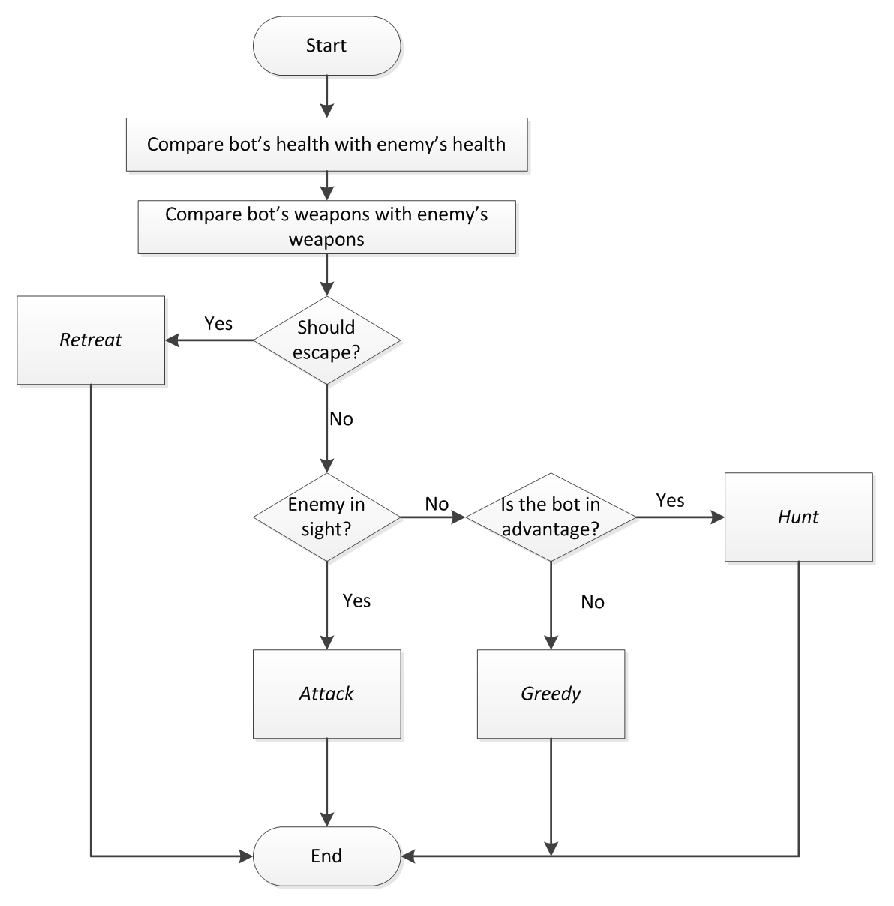
\includegraphics[scale=0.5]{imags/primary_states_flowchart.eps}
%   \caption{Primary States selection flow chart}
%   \label{fig:primary_states_flowchart}
%\end{figure}

%
%The \textit{Camp} state is not included because it is a special state with very particular conditions.
The comparisons and decisions required to choose the state are quite complex, because they consider several factors and situations that the human expert knows. For instance, the comparison of weapons depends on several parameters and weights, because of the existing balance between the power and usefulness of all of them, which could mean that a weapon is the best in a specific situation (different levels, hidden opponent, close/far enemy), but that weapon would be the worst on a different position. 

The AI engine (composed by a huge system of rules) at a time chooses the primary state, but while the bot is performing the actions associated to it, the engine continues checking conditions (for instance the timing of every item), receiving sensory information, checking the bot status, etc. This way, a secondary state can be also set. However the engine can stop and change, at any time, both the primary and/or the secondary state, depending of the conditions, received information and status, giving an extra `flexibility' level to the FSM.

As a general summary, the bot tends to be defensive if its health is lower than the enemy's, unless the latter has a critical health level, so the bot will attack him to win a frag. In similar health conditions the attitude depends on the weaponry (in comparison with the enemy's weapons). If the bot's health is good, it is quite aggressive.
%However, there are considered several conditions and situations which could change the states and actions to perform. For example, the difference in levels.
%The \textit{E-Bot} general flow chart can be seen in Figure \ref{fig:e-bot_flowchart}.
%
%\begin{figure}[htb]
%   \centering
%   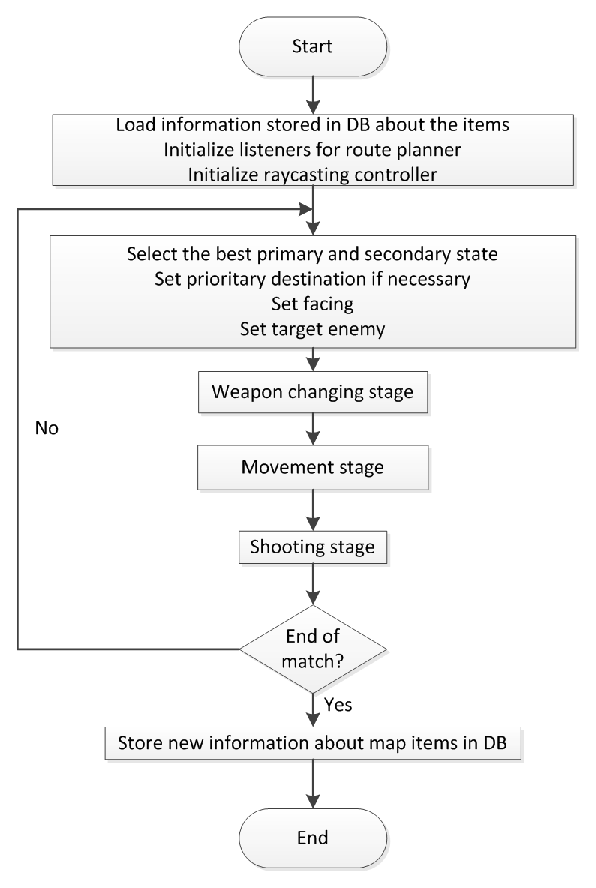
\includegraphics[scale=0.6]{imags/expert_flowchart.eps}
%   \caption{\textit{E-Bot} general flow chart. The route planner controls the navigation around the map, while the raycasting controller traces vision lines for avoiding obstacles and seeing enemies.}
%   \label{fig:e-bot_flowchart}
%\end{figure}
%
%One bot, during a game, changes its current state depending on some factors present in its surroundings and depending on its own status and location. 
%That is, the states transitions strongly depend on a number of parameters which determine the final behaviour of the bot, since most of them are thresholds depending on which, the bot state changes (for instance, the distance to an enemy or the bot's health level). 
%These variables can be related to the individual behaviour, but some of them are also devoted to model the behaviour of the bot inside a team.
%
%In addition, the thresholds are typically compared with hard-coded values inside the source code of the bot's AI.
%This way, the state changing (and the power of the bot's AI) finally depends on some constant values.

The value of the expert bot has been tested in an experiment, consisting in four different \textit{1 vs 1 - Death Match} combats against a standard UT2K4 game bot, held in two different maps. The bots have been fighting, respecting championship rules, during 15 minutes. The results of every match as well as the average are shown in Table \ref{tab:e-bot_results}.
%
\vspace{-0.1cm}
\begin{table}[htp]
\centering
{\footnotesize
\begin{tabular}{|l|c|c|}
\hline
\textit{Map} & \textit{E-Bot} & \textit{StdBot}\\
\hline
\textit{DM-Ironic} & 13 (m1), 26 (m2) & 6 (m1), 8 (m2)\\
\textit{DM-Idoma} & 23 (m1), 25 (m2) & 15 (m1), 8 (m2)\\
\hline
Average & 21.75 & 9.25\\
\hline
\end{tabular}
\caption{Scores (number of frags) of the test fights between \textit{E-Bot} and a Standard UT2K4 bot in the hardest difficulty (\textit{StdBot}). Match 1 (m1) and 2 (m2) in every map.
\label{tab:e-bot_results} }
}
\end{table}
\vspace{-0.6cm}

As it can be seen \textit{E-Bot} outperforms the standard game bot, even in the hardest difficulty level, which is a challenge for a medium level player. 


%%%%%%%%%%%%%%%%%%%%%%%%%%%%%%   EVOLUTIONARY BOT  %%%%%%%%%%%%%%%%%%%%%%%%%%%%%
\vspace{-0.3cm}
\section{Evolution of the UT2K4 Expert Bot}
\label{sec:evolution}
\vspace{-0.1cm}

Following previous approaches \cite{cole_GAtuning_cec2004,Mora_Unrealbot_EVO2010,Mora_UnrealTeams_CIG2010}, the expert bot will be improved. To this end, the set of parameters which act as thresholds, weights, priorities and conditions, and which finally determine the final behaviour of the bot, will be optimized by means of a Genetic Algorithm (GA)\cite{GA_Goldberg89}, which can evolve their values searching for the best combination, i.e. the set of values which performs better in a battle.
Following this idea, we have designed and tested a GA-based bot, named \textit{GE-Bot}\footnote{The source code of both \textit{E-Bot} and \textit{GE-Bot} can be downloaded from\\ 
{\small \url{https://github.com/franaisa/EvolutionaryBot}} under a GPL license.}, following different approaches.


%--------------------------------------------------------------------
\vspace{-0.3cm}
\subsection{First approach: chromosome-143}
\label{subsec:first_GA}
\vspace{-0.2cm}

In this approach the \textit{chromosome scheme} has 143 genes, grouped in six different blocks: having 2 genes for health levels, 3 genes for distance, 5 genes to value the risk, 1 gene for time to see an enemy, 6 genes for items priority, and 126 genes related to weapons selection.
%, as shown in Table \ref{tab:chromosome143}.
%
%\begin{figure}[htb]
%   \centering
%   \includegraphics[scale=0.27]{imags/chromosome143.eps}
%   \caption{\textit{GE-Bot} 143 genes chromosome}
%   \label{fig:chromosome143}
%\end{figure}
%
%
%\begin{table}
%\centering
%{\footnotesize
%\begin{tabular}{|l|l|l|l|l|l|}
%\hline
%\multicolumn{1}{|c|}{$health$} & \multicolumn{1}{c|}{$distance$} & \multicolumn{1}{c|}{$risk$} & \multicolumn{1}{c|}{$time$} & \multicolumn{1}{c|}{$items$} & \multicolumn{1}{c|}{$weapons$} \\ 
%\multicolumn{1}{|c|}{2} & \multicolumn{1}{c|}{3} & \multicolumn{1}{c|}{5} & \multicolumn{1}{c|}{1} & \multicolumn{1}{c|}{5} & \multicolumn{1}{c|}{126} \\ 
%\hline
%\end{tabular}
%}
%\caption{\textit{GE-Bot} 143 genes chromosome. Number of genes grouped by blocks}
%\label{tab:chromosome143}
%\end{table}
%
%As it can be seen in the table there are six different blocks:
%\begin{itemize}
%    \item \textit{health}: levels to be defensive, offensive or neutral.
%    \item \textit{distance}: close, medium and far distances for choosing a weapon to attack and/or maintain the separation with the enemy.
%    \item \textit{risk}: number of health points that the bot could lose in an action.
%    \item \textit{time}: time to consider an enemy as lost (from the bot point of view).
%    \item \textit{items}: items priority for timing, i.e. which one is the most interesting for waiting its respawn.
%    \item \textit{weapon selection}: priority of using each weapon, considering distance, height and the situation of the bot with respect to the enemy.
%\end{itemize}

The \textit{fitness function} has been defined as:

\begin{footnotesize}
\begin{equation} \label{eq:fitness}
f=\left\{ \begin{array}{ll} 
3 + (damP/damR) & \textit{if (frags + 1) = deads}\\

      (2 \cdot frags - deads) + (damP/damR) & \textit{if frags $>$ deads}\\

      (3/2) + (damP/damR) & \textit{if frags = deads}\\

      frags/deads & \textit{if frags $<$ deads}\\
\end{array} \right.
\end{equation}
\end{footnotesize}

Where $frags$ is the number of enemy kills  the bot has obtained, $deads$ is the number of own deads, $damP$ is the total damage produced by the bot, and $damR$ is the total damage it has received.
This function rewards the individuals with a positive balance (more frags than deads) and a high number of frags. In addition individuals which perform a high amount of damage to the enemies are also rewarded, even if they have not got a good balance.

The \textit{evaluation of an individual} consists in setting the values of the chromosome in the \textit{E-Bot} AI engine, then a 1 vs 1 combat is launched between this and a standard \textit{E-Bot}. After the time limit defined, the fitness value is computed for the individual. There is a high pseudo-stochastic component in these battles, since the results do not depend completely on our bot, but also on the enemy's actions which we cannot control. Thus, the fitness function is considered as noisy \cite{Mora_noisy_jcst}, since an individual could be valued as good in one combat, but yield very bad results in another match. 
%In order to (partially) avoid this issue, some other evaluations (combats) are performed for every individual, being the final fitness value an average.

An \textit{elitist selection mechanism} has been applied, remaining the best four individuals in the next population. The rest of population is considered as parents.

The \textit{uniform crossover} operator (every gene of a descendent has the same probability of belonging to each one of the parents) has been applied in two steps: on the one hand it is used with the elite, yielding two descendents by combining the best individual with a random one in the best four chosen. On the other hand, the rest of the offspring is formed as a random combination of the rest of parents (in pairs). Finally, four random individuals are included in the population (they substitute the four worse) to add diversity.

The \textit{mutation mechanism} is performed on every descendent. It changes with a probability $1/chromosome\_size$ the value of every gen in a $\pm$10\% rate.

%Due to the high computational time the evolution consumes (mainly for the expensive evaluation function), a database is used for storing the status in every moment (individuals, evaluations, chromosome values, etc). It lets the user to continue the execution in case an unexpected error occurs (a machine fail, for instance), or after a programmed pause.

Some experiments were conducted to test this approach for the \textit{GE-Bot}. All of them (and next) have been conducted in the map DM-Ironic, since it is one of the most used maps in competitions, and has a design that offers almost any possible fighting situation: different levels, hidden zones, viewpoints and camping areas.

%
%\textcolor{red}{Firstly, the fitness function utility was proved, checking how the noise affected it. To this end, there were conducted 30 battles between a standard \textit{E-Bot} and three different customized (by the expert) bots to perform as good, regular and bad players.
%The results can be seen in Figure XX, showing an average good performance of the function.}
%
Firstly, the algorithm is tested considering as parameter setting: \textit{30 generations, 30 individuals, and 15 minutes every evaluation}, taking 10 running days. 
% Since this is a preliminary study and due to the high computational cost, just one run has been performed in this experiment.

%\begin{figure}[h]
%   \centering
%      \begin{tikzpicture}
%      \begin{axis}[
%         xlabel = Generacion,
%         ylabel = Fitness,
%         height = 9cm,
%         width = \linewidth
%      ]
%         \addplot[color = green, mark = x] coordinates {
%            (0, 15.1154)
%            (1, 23.4727)
%            (2, 33.4624)
%            (3, 19.5677)
%            (4, 11.1562)
%            (5, 45.4286)
%            (6, 10.5532)
%            (7, 13.0142)
%            (8, 15.6562)
%            (9, 16.1761)
%            (10, 18.087)
%            (11, 24.2727)
%            (12, 16.0153)
%            (13, 21.4681)
%            (14, 16.3348)
%            (15, 22.8352)
%            (16, 37.4444)
%            (17, 14.2312)
%            (18, 25.8605)
%            (19, 18.2781)
%            (20, 17.5647)
%            (21, 21.2394)
%            (22, 12.7055)
%            (23, 12.8618)
%            (24, 18.1221)
%            (25, 11.9517)
%            (26, 15.7349)
%            (27, 14.8165)
%            (28, 23.2215)
%            (29, 35.8356)
%         };
%         \addplot[color = gray, mark = x] coordinates {
%            (0, 1.60761)
%            (1, 2.01046)
%            (2, 3.64447)
%            (3, 3.15367)
%            (4, 1.61795)
%            (5, 3.7038)
%            (6, 0.891528)
%            (7, 1.32407)
%            (8, 2.43088)
%            (9, 1.94315)
%            (10, 2.47632)
%            (11, 2.98062)
%            (12, 2.4111)
%            (13, 2.82592)
%            (14, 2.37317)
%            (15, 2.29631)
%            (16, 3.50208)
%            (17, 2.27868)
%            (18, 3.12227)
%            (19, 1.84965)
%            (20, 2.47032)
%            (21, 1.90173)
%            (22, 1.57507)
%            (23, 1.96816)
%            (24, 1.61766)
%            (25, 1.61133)
%            (26, 2.0657)
%            (27, 1.64193)
%            (28, 6.00056)
%            (29, 3.31837)
%         };
%         \legend{Elitista, Mejor Fitness, Media}
%      \end{axis}
%   \end{tikzpicture}
%   \caption{30 generaciones, 30 individuos, 15 minutos por evaluation.}
%   \label{fig:experiment_1}
%\end{figure}
%
Figure \ref{fig:exp1} shows the best and average fitness evolution in the run, considering one (left side) and three (right side) evaluations per individual.
%
\begin{figure}[htb]
   \centering
   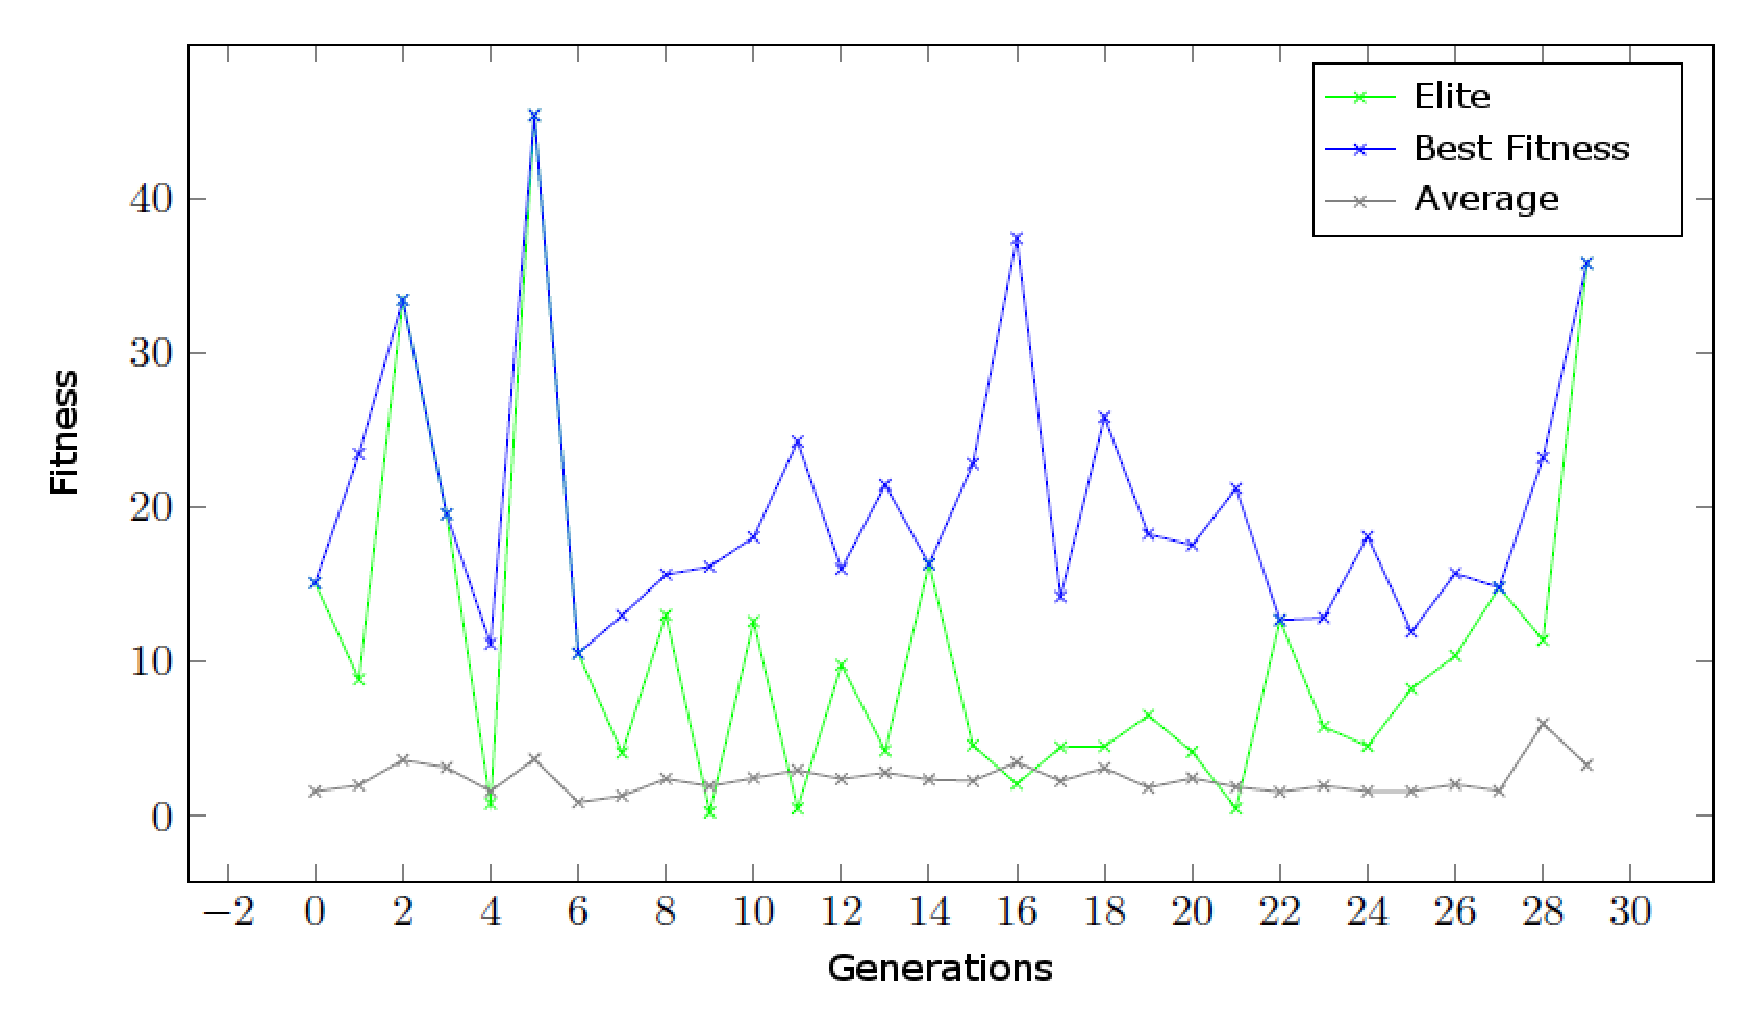
\includegraphics[scale=0.2]{imags/exp1_c143-30g-30i-15min.eps}
   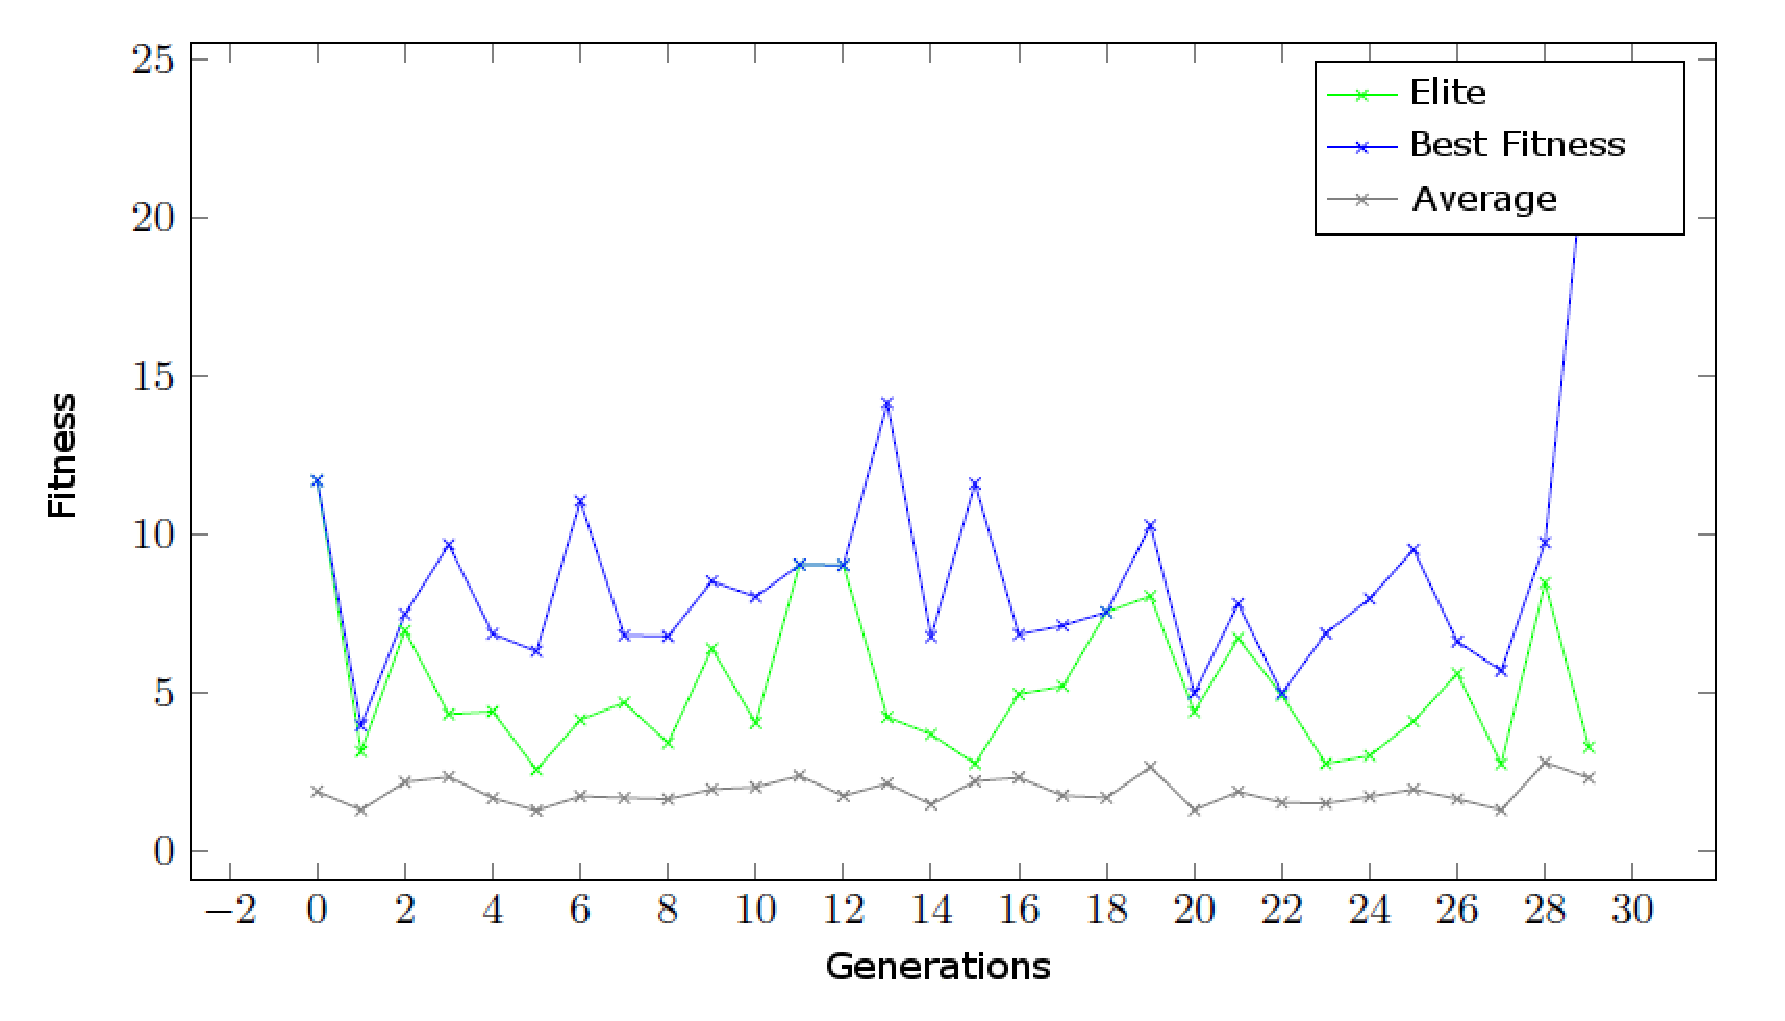
\includegraphics[scale=0.2]{imags/exp2_c143-30g-30i-15min-3evs.eps}
\vspace{-0.3cm}
   \caption{Fitness evolution of the best, elite and average in 30 generations for the first approach of GE-Bot (143 genes chromosome, 1 evaluation (left) and 3 evaluations (right) per individual).}
   \label{fig:exp1}
\end{figure}

As it can be seen on the left subfigure, the evolution is highly noisy, as commented when the fitness function was defined, due to the pseudo-stochasticity of combats. In order to deal with this effect, some evaluations (different matches) per individual have been performed, as it is recommended \cite{Mora_noisy_Genebot_EVO2012}. This second experiment has taken one month of computational time and is plotted on the right side subfigure. An improvement in the fitness evolution tendency is shown.
%
%\begin{figure}[htb]
%   \centering
%   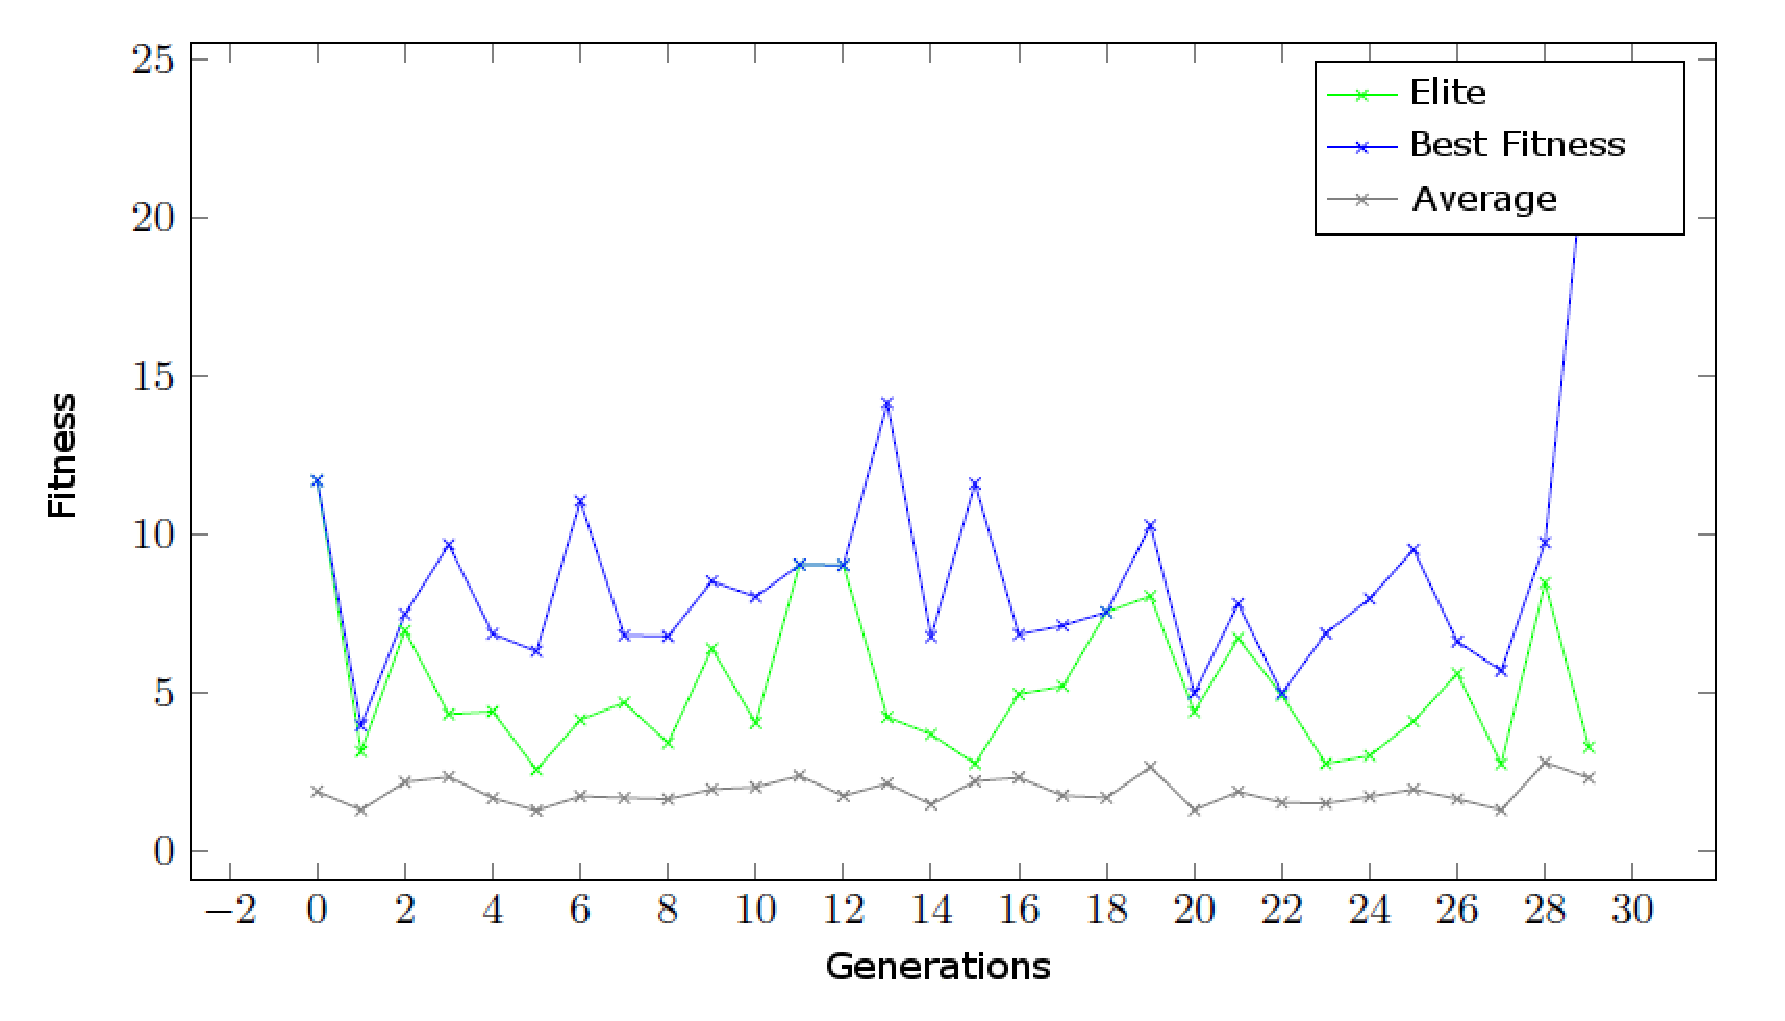
\includegraphics[scale=0.3]{imags/exp2_c143-30g-30i-15min-3evs.eps}
%   \caption{Fitness evolution of the best, elite and average in 30 generations for the first approach of GE-Bot (143 genes chromosome) with 3 evaluations per individual.}
%   \label{fig:exp2}
%\end{figure}

The best fitness graphs proved the noise nature of the function, so even considering three matches for every evaluation, and having followed an elitist scheme, the best values oscillate without a clear tendency. The average results show a lightly improvement tendency, which let us think in a good (but slow) evolution and improvement of individuals (parameters) or results.
The reasons of these light tendencies and high oscillations might be two: first reason could be the chromosome length, since the evolution of 143 genes might take much more generations; the second reason could be the inclusion of diversity enhancement mechanisms, such as the uniform crossover or the random generation of some individuals (which substitute the four worst). 

%--------------------------------------------------------------------
\vspace{-0.3cm}
\subsection{Second approach: chromosome-26}
\label{subsec:second_GA}
\vspace{-0.2cm}

Since the chromosome length implies a high number of generations (and so, huge computational time) are required for a good optimization process, the \textit{chromosome scheme} was redefined considering 26 genes, by reducing the weapons block to just 9 genes (one associated to the priority of each weapon). This representation is less precise from the expert's AI performance point of view, but with a more approachable size.
The rest of the algorithm terms and operators remained the same.
Results are presented in Figure \ref{fig:exp3} (two runs of ten), with a different parameter setup, due to the expected computational time reduction, so, in order to perform a more complete evolution, \textit{the number of generations has been increased to 50, being the population again 30 individuals and considering this time 5 minutes for evaluating every individual}. The running time of this experiment has been 5 days per run.
%
\begin{figure}[htb]
   \centering
   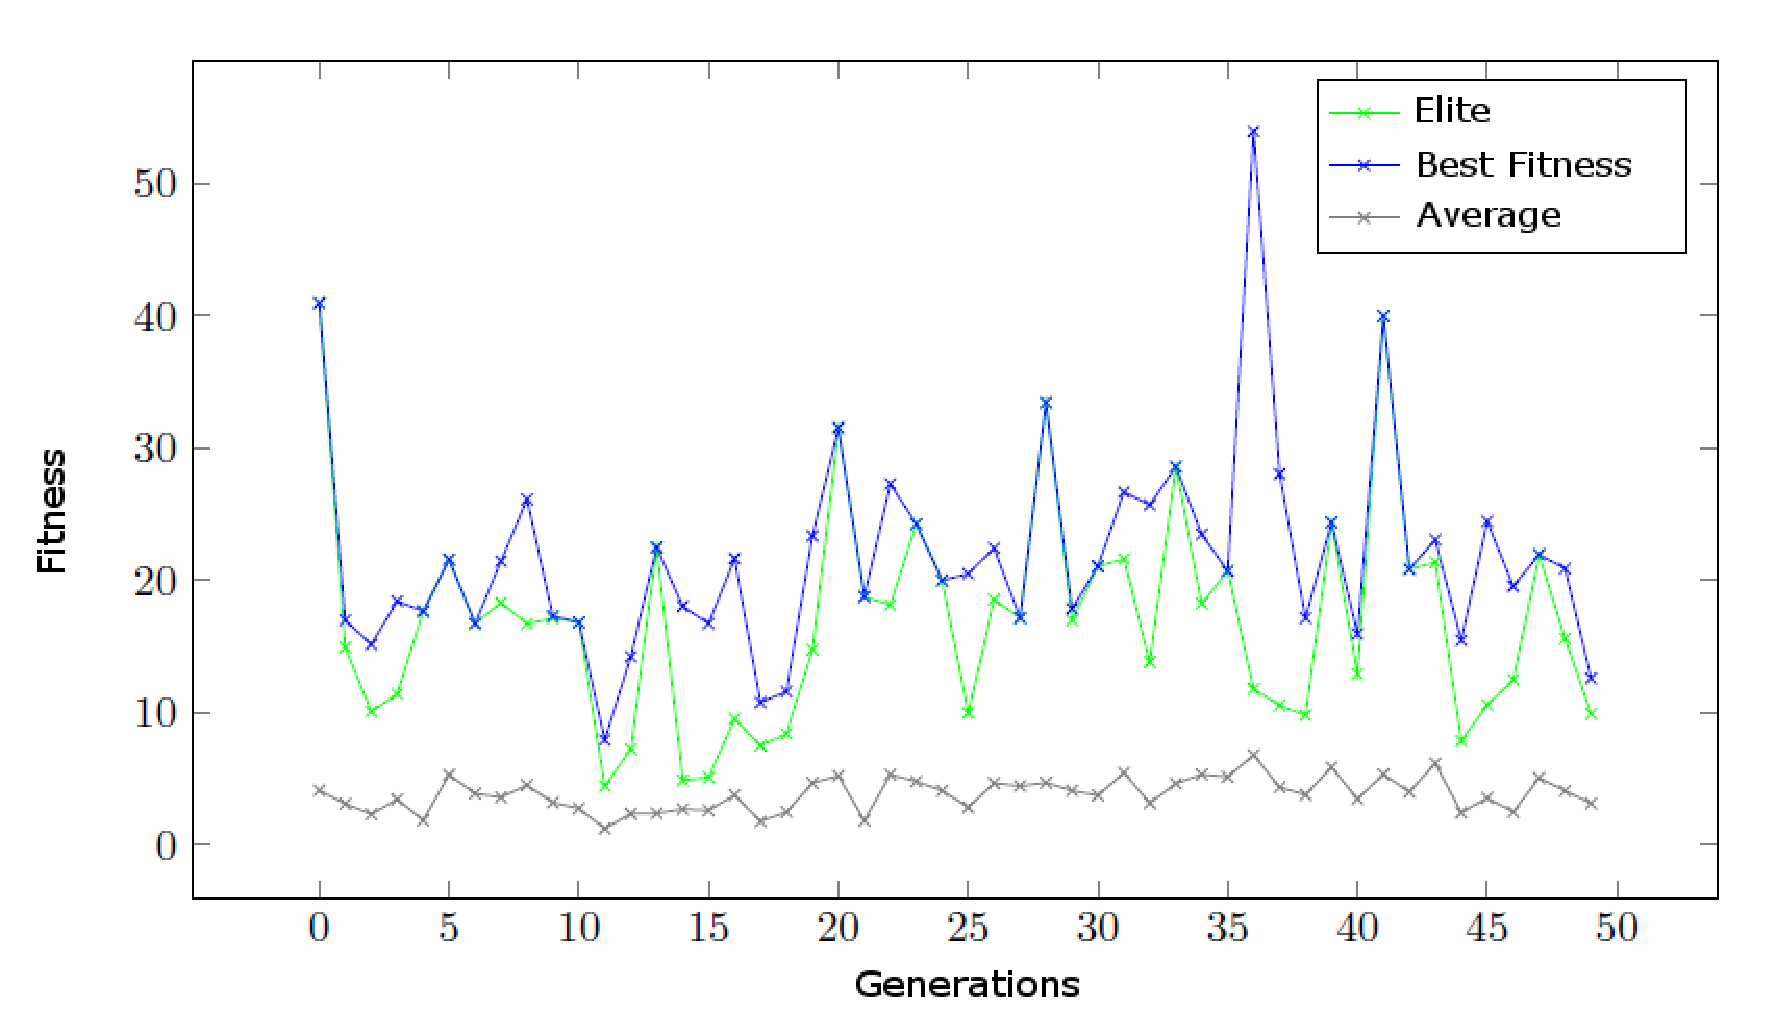
\includegraphics[scale=0.2]{imags/exp3_c26-50g-30i-5mins-1.eps}
   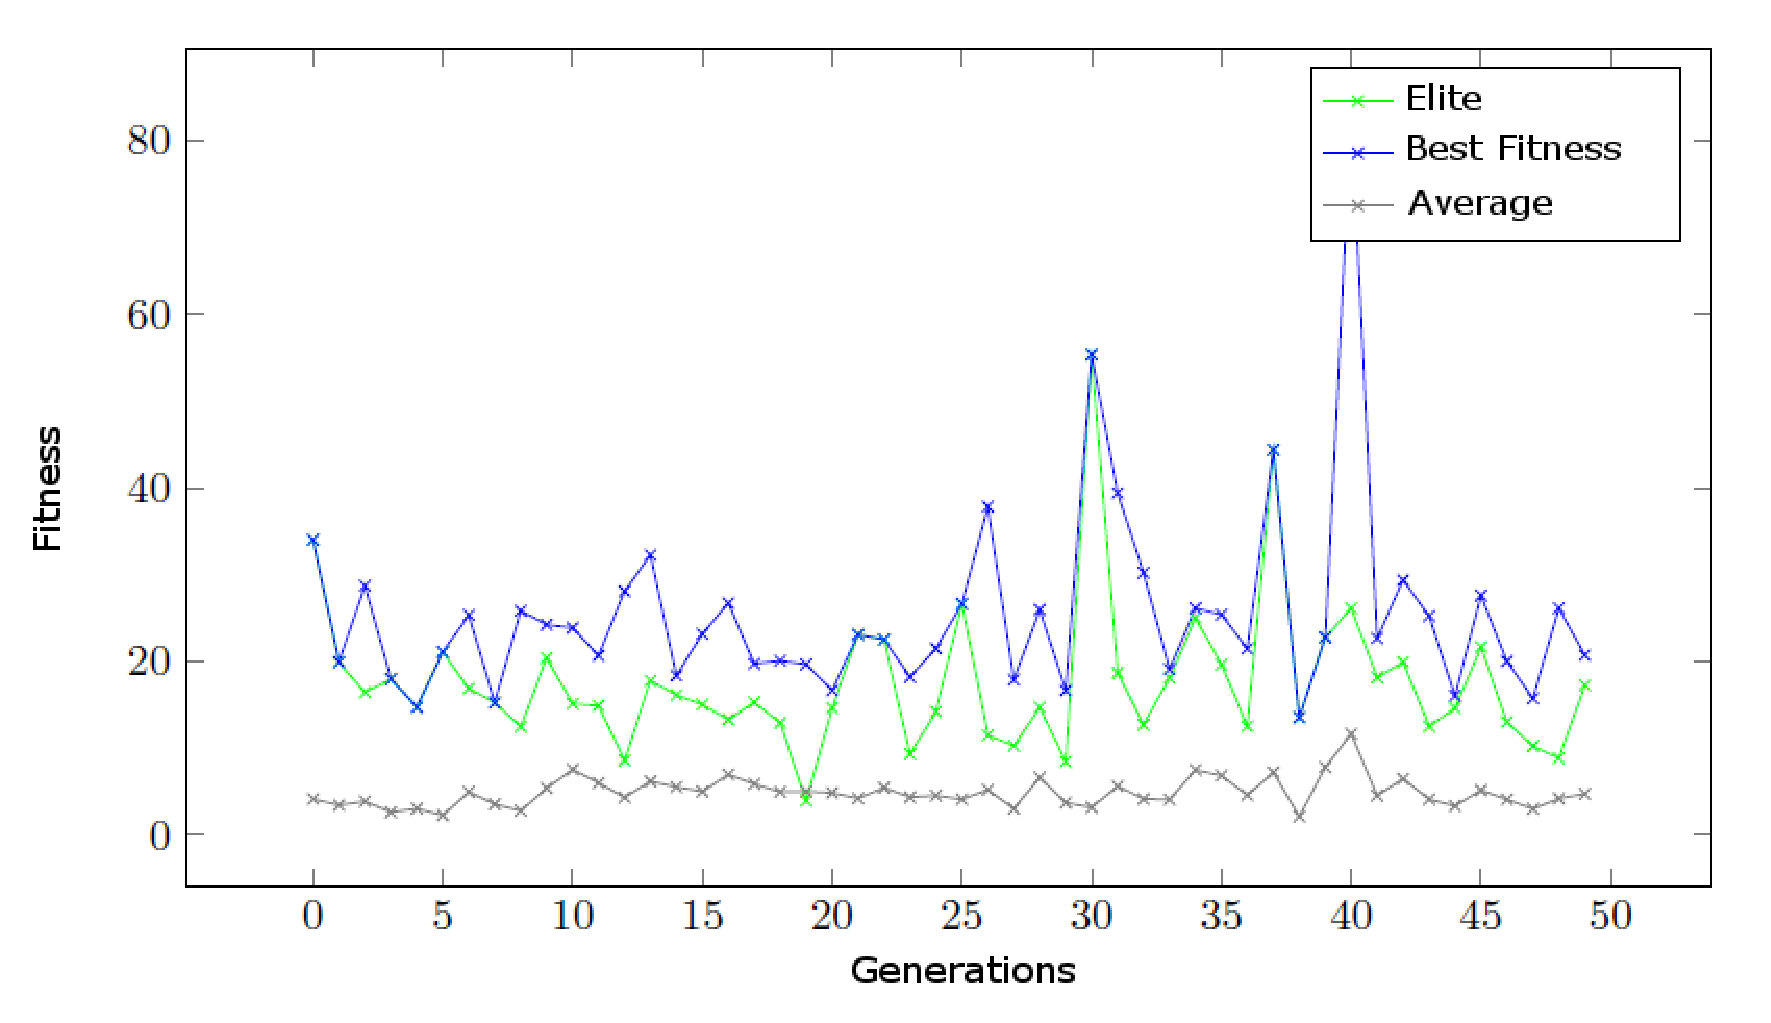
\includegraphics[scale=0.2]{imags/exp3_c26-50g-30i-5mins-2.eps}
\vspace{-0.3cm} 
  \caption{Fitness evolution of the best, elite and average in 50 generations for the second approach of GE-Bot (26 genes chromosome). Two different runs.}
   \label{fig:exp3}
\end{figure}

As it is shown, there are again fluctuations and light improving tendencies. The oscillations seem to be lighter, but what is happening is that the resulting values have been reduced (due to the shorter battle time). The average fitness tendency on the other hand is less clear this time. Thus, the reduction in the evaluation time just has meant an improvement in the computational cost.

%--------------------------------------------------------------------
\vspace{-0.3cm}
\subsection{Third approach: fitness and operators redefinition}
\label{subsec:third_GA}
\vspace{-0.2cm}

According to the second conclusion reached by the end of Subsection \ref{subsec:first_GA}, the evolution in this problem is quite difficult, so it would be recommended the implementation of mechanisms to increase the exploitation of solutions rather than increasing diversity (as it has been done). 

Firstly, the fitness function has been redefined in order to take into account more elements of the individual/bot performance during a match, i.e. the most important items for survive and the best weapons for our bot (the most useful according to the defined FSM). They have been included in some terms of the evaluation function as follows:

\begin{footnotesize}
\begin{equation} \label{eq:fitness_complex}
f=\left\{ \begin{array}{ll} 

(frags - deads) + s2 + \frac{s1}{2} + \frac{tS/10}{d + 1}\\ + \frac{tL/10}{d + 1} + \log ((damP-damR)+1) & \;\; \textit{if frags $\ge$ deads}\\
\\
\frac{frags}{deads} + s2 + \frac{s1}{2} + \frac{tS/10}{d + 1}\\ + \frac{tL/10}{d + 1} + \log ((damP-damR)+1) & \;\; \textit{if frags $<$ deads}\\

\end{array} \right.
\end{equation}
\end{footnotesize}

Where $frags$, $deads$, $damP$ and $damR$ are the same as in Equation \ref{eq:fitness}. $s1$ and $s2$ refers respectively to the number of Shields and Super Shields the bot has picked up. $tS$ is the time the bot has used the Shock Rifle, and $tL$ refers to the time it has used the Lightning Gun.
The term frags is the most important and the rest are weighted to have lower relevance.

The GA scheme has been changed to a stationary approach in order to increase the selective pressure and get a higher convergence factor. Thus the best 15 individuals are considered for the new population. They also are one of the parents for generating the offspring and the other parents are selected using a probability roulette wheel from the rest of population.
The crossover and mutation operators remains the same as in the other approaches.

Figure \ref{fig:exp4} shows the results of two runs (of ten), considering the same parameter configuration as in the last approach.
%
\begin{figure}[htb]
   \centering
   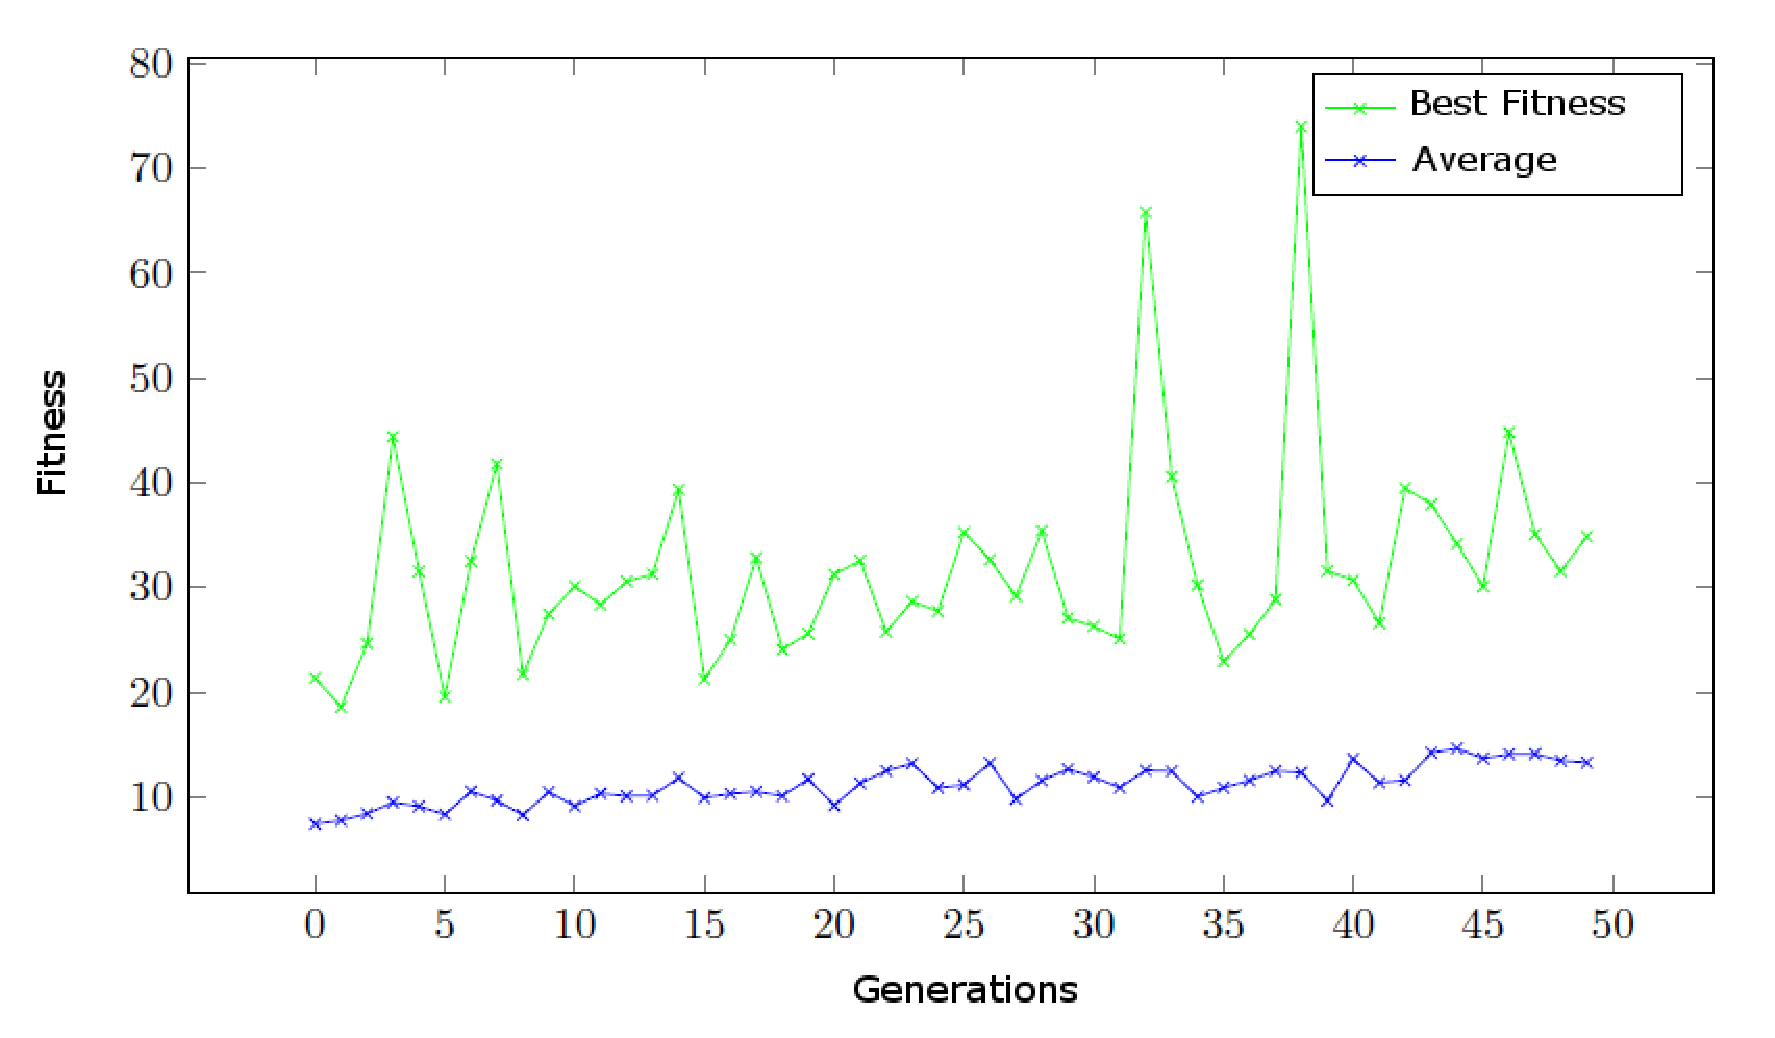
\includegraphics[scale=0.2]{imags/exp4_c26-50g-30i-5mins-fitcomplex-1.eps}
   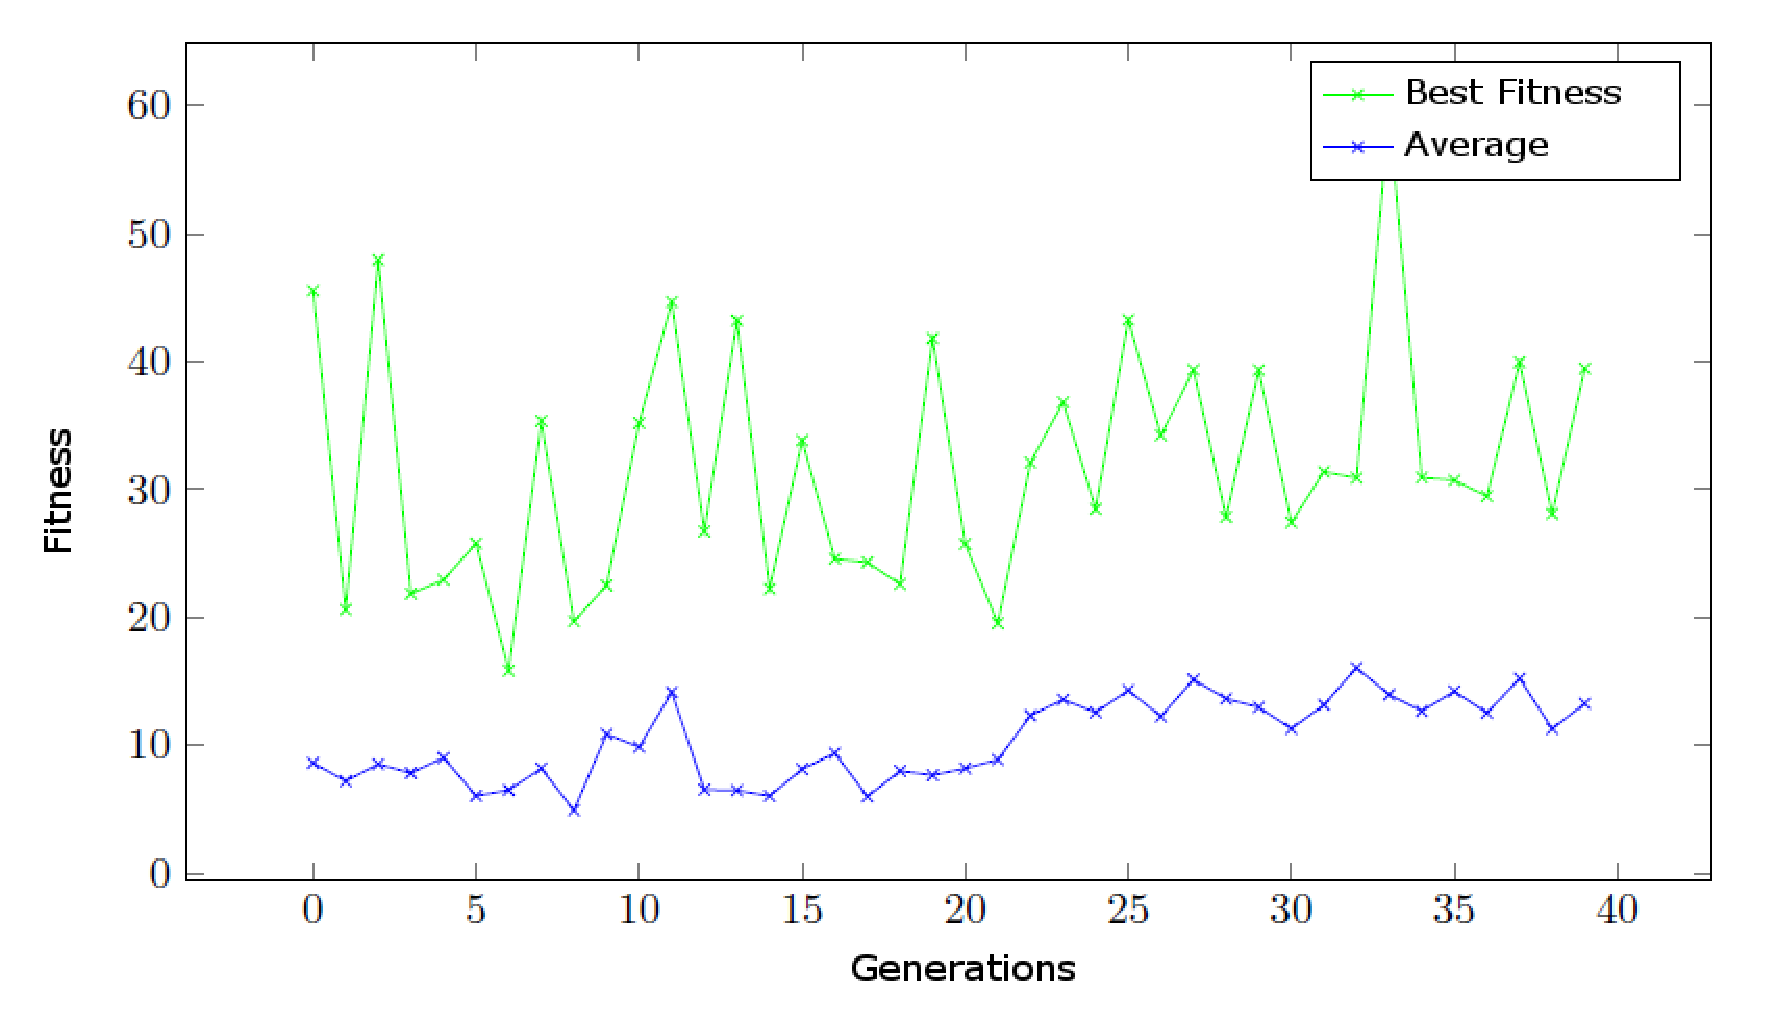
\includegraphics[scale=0.2]{imags/exp4_c26-50g-30i-5mins-fitcomplex-2.eps}
\vspace{-0.3cm}
   \caption{Fitness evolution of the best, and average in 50 generations for the third approach of GE-Bot (26 genes chromosome, complex fitness function and stationary scheme).}
   \label{fig:exp4}
\end{figure}

As it can be seen, the results are better than in previous approaches, showing a `softer' fitness tendency (with less fluctuations), and a clear improving, with the generations, in the average results.


%%%%%%%%%%%%%%%%%%%%%%%%%%%%%%   EXPERIMENTS  %%%%%%%%%%%%%%%%%%%%%%%%%%%%%%%
%
%\section{Experiments and Results}
%\label{sec:experiments}
%



% Subsecci�n o nueva secci�n aqu�? - JJ
% ocupar�a mucho m�s...

%The following experiments are aimed to test the value of the evolutionary approach. 
%Some tests with \textit{GE-Bot} have been performed, applying different configurations in chromosome length, number of generations, and in the evaluation function (number of matches and time of everyone).
%The parameters considered are shown in Table \ref{tab:ga-params}. Most of them have been set starting from standard GA ones, and tuning through systematic experimentation.
%
%\begin{table}[htp]
%\centering
%\caption{Parameters of GA (used in \textit{GE-Bot}).
%\label{tab:ga-params} }
%\begin{tabular}{|l|c|}
%\hline
%\textit{Number of individuals} & 30\\
%\textit{Chromosome length} & 26, 143\\
%\textit{Mutation probability} & 1/26, 1/143 \\
%\textit{Mutation rate} & $\pm$10\% \\
%\textit{Number of generations} & 30, 50 \\
%\textit{Time limit per chromosome} & 2, 3, 5 minutes \\
%\textit{Number of evaluations per chromosome} & 1, 3 \\
%\hline
%\end{tabular}
%\end{table}
% 
%Looking at the values it can be seen that the evaluation of one individual takes, depending on the configuration, from 2 to 15 minutes (3 times x 5 minutes), which means that each experiment has spend from 5 to 19 days. Since this is a preliminary study and due to the high computational cost, just one run has been performed in some experiments.

%It is important to notice that the \textit{opponent to evaluate every
%  individual} of \textit{GE-Bot} is always one
%\textit{E-Bot}. Moreover the map DM-Ironic, has been considered for
%all runs, because it is one of the most famous maps, used in
%competitions and with a design that offers almost any possible
%fighting situation: different levels, hidden zones, viewpoints
%and camping areas.

%---------------------------------------------------------------

%The first experiment with \textit{GE-Bot}, has performed one run with 30 generations, using the initial scheme with 143 genes per chromosome and doing 3 battles (of 5 minutes each) for evaluating every individual. The associated fitness to the individual is the average of the 3 values (each one obtained through Equation \ref{eq:fitness}). As stated, the objective of this evaluation scheme based in repetitions is trying to deal with the noisy nature of the fitness function \cite{Mora_noisy_Genebot_EVO2012}, since the results for the same individual evaluation may change from time to time, yielding good or bad values depending on the battle events and on the opponent's actions (his behaviour, and even our bot's are non-deterministic).
%
%Figure \ref{fig:GE-Bot_30-143-3t-5m} shows the best and average fitness (of the whole population) evolution in the run. 
%
%\begin{figure}[ht]
%\begin{center}
%\includegraphics[scale=0.235,angle=-90]{imags/best30gen143genes.eps}
%\includegraphics[scale=0.235,angle=-90]{imags/average30gen143genes.eps}
%\caption{Best (left) and average (right) fitness evolution in the experiment with 30 generations, 143 genes per chromosome and 3 evaluations per individual (5 minutes each). 
%\label{fig:GE-Bot_30-143-3t-5m}}
%\end{center}
%\end{figure}
% EStos dos gr�ficos o los pones juntos o los quitas. No aportan nada,
% y ocupan demasiado espacio. A qui�n se le ha ocurrido poner en
% gr�ficos diferentes el mejor y la media? - JJ
% Era por poner algo, ya que no hay resultados 'tangibles'. Si los pon�amos juntos no se ve una mielda porque se mueven en rangos distintos. Lo dejamos para la versi�n final.

%As it is plotted in the figure (left side), the best fitness graph proved the noise nature of the function, so even considering 3 matches for every evaluation, and having followed an elitist scheme, the best values oscillate without a clear tendency. The average results (on the right side plot) show a lightly improvement tendency, which let us think in a good (but slow) evolution and improvement of individuals (parameters) or results.
%The reasons of these light tendencies and high oscillations might be two: first the inclusion of diversity enhancement mechanisms, such as the uniform crossover or the random generation of some individuals (which substitute the four worst); the second reason could be the chromosome length, since the evolution of 143 genes might take much more generations.

%---------------------------------------------------------------

%Thus as commented in Section \ref{sec:evolution}, we decided to implement another chromosome scheme, less precise from the expert's AI performance point of view, but with a smaller and more approachable size. In addition and with the aim of reducing the computational cost, the battle time has been reduced to 2 minutes.
%So there have been considered 30 generations with 26 genes per chromosome performing 3 battles (of 2 minutes each) for evaluating every individual.
%Figure \ref{fig:GE-Bot_30-26-3t-2m} plots the graphs for the best and average fitness evolutions.
%
%\begin{figure}[ht]
%\begin{center}
%\includegraphics[scale=0.235,angle=-90]{imags/best30gen26genes.eps}
%\includegraphics[scale=0.235,angle=-90]{imags/average30gen26genes.eps}
%\caption{Best (left) and average (right) fitness evolution in the experiment with 30 generations, 26 genes per chromosome and 3 evaluations per individual (2 minutes each).
%\label{fig:GE-Bot_30-26-3t-2m}}
%\end{center}
%\end{figure}
% EStos dos gr�ficos o los pones juntos o los quitas. No aportan nada,
% y ocupan demasiado espacio - JJ

%As it is shown, there are again fluctuations and (very) light improving tendencies. The oscillations seem to be lighter, but what is happening is that the resulting values have been reduced (due to the shorter battle time). The average fitness tendency on the other hand is less clear this time. Thus, the reduction in the evaluation time just has meant an improvement in the computational cost (almost half of time).

%---------------------------------------------------------------

%Finally, we have tested the short chromosome scheme with a higher number of generations (50), but performing just a battle (of 5 minutes) for evaluating an individual. To better check the approach value 10 runs have been performed.
%The graphs can be seen in Figure \ref{fig:GE-Bot_50-26-5m}, where the graphs of the average values are plotted along with the standard deviation (of the 10 runs) for both the best fitness and the average fitness of the whole population.
%
%\begin{figure}[ht]
%\begin{center}
%\includegraphics[scale=0.235,angle=-90]{imags/best50gen26genes10runs.eps}
%\includegraphics[scale=0.235,angle=-90]{imags/average50gen26genes10runs.eps}
%\caption{Best (left) and average (right) fitness evolution in the experiment with 50 generations, 26 gene length and 5 minutes evaluations per individual. 10 runs.
%\label{fig:GE-Bot_50-26-5m}}
% Las desviaciones t�picas son para cuantas ejecuciones? - JJ
% lo pone 2 l�neas m�s arriba, jeje
%\end{center}
%\end{figure}
%
%Again, the graphs show fluctuations in the results, which can be also contrasted looking at the high standard deviations in both graphs. This means that the noisy nature of the fitness is not well controlled just with the repetition of battles and more `aggressive' methods should be employed. 
%The tendency in the average fitness seems to appear again as in the first experiment, and the values, that can be compared which the first (Figure \ref{fig:GE-Bot_30-143-3t-5m}) since the time for a battle is the same, are lightly better in this experiment. The reason is the smaller chromosome length, which is easier evolved (and improved).

%However the evolution in this scope is quite difficult, so it would be recommended the implementation of mechanisms to increase the exploitation of solutions rather than increasing diversity (as it is done here). For instance a stationary model (almost all the population is maintained from one generation to another) could be considered.

%---------------------------------------------------------------
\vspace{-0.3cm}
\section{Expert Bot versus Evolved Bots}
\vspace{-0.1cm}

A last test has been performed confronting the best individuals of the \textit{GE-Bot} approaches against \textit{E-Bot}, since they have been optimized for beating it (they have fought against it during the evolution).
The average results of four matches are shown in Table \ref{tab:ge-bot_vs_e-bot_results}. They have been held in the same two maps and for 15 minutes each.
\vspace{-0.3cm}
%
\begin{table}[htp]
\centering
{\footnotesize
\begin{tabular}{|l|ll|l|}
\cline{2-3}
\multicolumn{1}{l|}{} & \multicolumn{2}{c|}{Score} & \multicolumn{1}{l}{} \\ 
\hline
GE-Bot: 143chr-30gen-3evals & 4.2 & 13.2 & E-Bot \\ 
GE-Bot: 26chr-50gen-1evals & 15.3 & 7.8 & E-Bot \\ 
GE-Bot: 26chr-50gen-1evals-complexfitness & 17.5 & 6.2 & E-Bot \\ 
\hline
\end{tabular}
\caption{Average scores (number of frags) of the test fights between the three approaches of \textit{GE-Bot} versus \textit{E-Bot}. 4 battles in two maps: DM-Ironic and DM-Idoma.
\label{tab:ge-bot_vs_e-bot_results} }
}
\end{table}
\vspace{-0.8cm}

The results show that the \textit{GE-Bots} with a higher number of
generations and smaller chromosome perform better than the one with
the higher length. This result should be expected, since the
chromosome length is a key factor in the evolution, because it defines the search space size, so long individuals need a higher number of generations. 
In this case, we just have performed (due to the huge computational time required) 30 generations for 143 genes which are clearly insufficient, according to the experiments results. 
The evolved for longer \textit{GE-Bots} (50 generations) yield a very
good performance beating \textit{E-Bot} in average. Finally, the last approach considering the complex fitness function performs better than the rest, because it is less influenced by the noisy nature of the evaluation function due to the consideration of additional (and important)factors to compute it.

%Moreover, the consideration of just one `long time' evaluation (5 minutes) performs better than three `short time' ones (2 minutes), because in the latter the individuals have not enough time to do valuable actions.
% Deber�ais decir algo de que evaluar con 5 minutos da mejores
% resultados que tres evaluaciones con dos minutos - JJ
% Hecho - Antonio

%---------------------------------------------------------------

%As an additional test, our expert (human) player fought some matches against \textit{E-Bot}, beating it always, so there still remain several point of improvement to create a high competitive bot. Among them, and according to the expert criterion, the bot movement must be highly improved, since the implementation which offers Pogamut does not include jumps, which in fact, are basic in an expert control.

%%%%%%%%%%%%%%%%%%%%%%%%%%%%%%  CONCLUSIONS  %%%%%%%%%%%%%%%%%%%%%%%%%%%%%%%
%
\vspace{-0.4cm}
\section{Conclusions and Future Work}
\label{sec:conclusions}
\vspace{-0.2cm}
%

In this work, a human-like bot for the First Person Shooter game Unreal Tournament\texttrademark~2004 (UT2K4) has been described. It models the expert knowledge of a Spanish high-level player so, its has been named Expert-Bot (\textit{E-Bot}). Its behaviour is based in a shape of finite state machine with two levels of states (primary and secondary), each of them with an associated priority for performing actions. This work flow is flexible, so the AI engine can alter/change it depending on the conditions or status (bot's or enemy's). Moreover, the bot uses a database for `learning' the maps, as a human player would do the first time it navigates around a new arena.
\textit{E-bot} has been designed for fighting in 1 vs 1 death match mode, considering the official competition rules.

Then a Genetic Algorithm (GA) has been implemented to improve the parameters (thresholds, weights, priorities) that the bot's AI considers in its behavioural rule system. The evolved expert bot, named \textit{GE-Bot} has been tested considering different approaches (chromosome length, number of generations, scheme, fitness function, crossover), along with an evaluation consisting in repeated battles which are rated once they have finished, for assigning an average fitness value to every individual in the population. The aim is to deal with the noisy nature of the fitness function, since it depends on the results of the battles, which can vary for the same individual from time to time, regarding to the situation in the map or the enemy's actions which we cannot predict.

Some experiments have been conducted, firstly proving that
\textit{E-Bot} outperforms the standard UT2K4 bots, even in the
hardest difficulty level. The result-to-effort ratio for
\textit{GE-Bot} is not very good, since the extremely high computation
time that every experiment takes (from 5 to 30 days), has limited the
number of generations and runs performed, so the improvement is not substantial. % Y las mejoras no son tan sustanciales? - JJ
% eso he puesto - Antonio
However, the results yielded show that the best approaches are those which consider a smaller chromosome size, and a higher number of generations, rather than wasting time in repeated evaluations. Moreover, the approach following a stationary scheme and a fitness function that considers items and weapons use gets the best performance and results. Both approaches have improved the results of \textit{E-Bot} and have beaten it in a set of test battles.
However, the evolution is not as good as desired and some repetitions of the evaluations could definitely help to improve this tendencies. We will consider this as the first future work line.

According to the expert's opinion, the bots do not perform as well as expected (from the behavioural point of view).
This way, another line of research will be the improvement of \textit{E-Bot} in its main flaw, the movement. Thus, the possibility of jumping must be included in its actions, in order to get a harder opponent (more difficult to kill).
Once the behaviour has been improved, several research could be conducted with regard to the evolutionary approaches, since the results in this paper can be considered as preliminary. A better noisy fitness dealing could be an interesting issue to address.

Finally, another option to study could be the optimization of \textit{E-Bot} for 
multiplayer and team modes, which are so far the most famous among the players.

%%%%%%%%%%%%%%%%%%%%%%%%%%%%%%   ACKNOWLEDGEMENTS %%%%%%%%%%%%%%%%%%%%%%%%%%%%%%

\section*{Acknowledgements}

This paper has been funded in part by projects P08-TIC-03903 (Andalusian Regional Government), and TIN2011-28627-C04-02 (Spanish Ministry of Science and Innovation), and by the FPU Grant 2009-2942.
The authors are very grateful to the Pogamut developers, specially to Michal Bida and Jakub Gemrot, by their dedication and support which has definitely aided to finish this work.

\vspace{-0.2cm}
\bibliographystyle{splncs}
\bibliography{unreal_expert}

\end{document}
